\documentclass[11pt]{article}

\usepackage[margin=1in]{geometry}
\usepackage{amsmath,amssymb,graphicx,multicol,array,enumerate,textcomp}
\usepackage{tikz}
\usepackage{pgfplots}
\pgfplotsset{compat=1.18}
\usetikzlibrary{arrows.meta,calc}

\newcommand{\usd}{\text{\$}}
\newcommand{\CA}{\text{CA}}
\newcommand{\dd}{\text{DD}}

\newenvironment{problem}[2][Problem]{\begin{trivlist}
\item[\hskip \labelsep {\bfseries #1}\hskip \labelsep {\bfseries #2.}]
\leavevmode\par
}{\end{trivlist}}

\begin{document}

\title{Problem Set 7}
\author{Joe White\\ECO 442}
\date{\today}
\maketitle

% =========================================================
\begin{problem}{1}

Using the short-run goods-market setup:
\[
D = C(Y-T) + I + G + \CA\!\left(\frac{EP^*}{P},\,Y-T\right),
\qquad
Y = D\!\left(\frac{EP^*}{P},\,Y-T,\,I,\,G\right).
\]
In the short run, $P$ and $P^*$ are fixed.

\vspace{0.5em}
\begin{enumerate}[(a)]
\item \textbf{Goods market (SR)}

A tax increase reduces disposable income:
\[
T\uparrow \Rightarrow (Y-T)\downarrow \Rightarrow C(Y-T)\downarrow.
\]
Lower disposable income also reduces imports, which tends to improve the current account:
\[
(Y-T)\downarrow \Rightarrow \CA\!\left(\frac{EP^*}{P},\,Y-T\right)\uparrow.
\]
Overall, aggregate demand falls at a given $Y$, so the $D$ schedule shifts down/left and equilibrium output falls.

\begin{center}
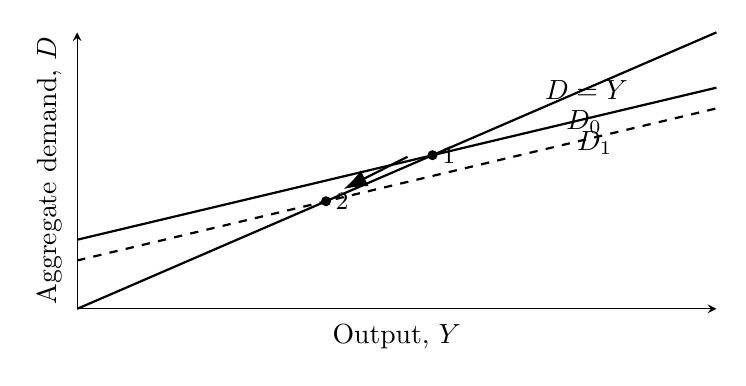
\begin{tikzpicture}
\begin{axis}[
  width=0.80\textwidth, height=0.42\textwidth,
  axis lines=left,
  xmin=0, xmax=12, ymin=0, ymax=12,
  xtick=\empty, ytick=\empty,
  xlabel={Output, $Y$},
  ylabel={Aggregate demand, $D$},
  clip=false
]

% 45-degree line
\addplot[domain=0:12, samples=2, thick] {x};
\node[anchor=west] at (axis cs:8.6,9.5) {$D=Y$};

% AD initial: D0 = a0 + bY, with b<1
\addplot[domain=0:12, samples=2, thick] {3.0 + 0.55*x};
\node[anchor=west] at (axis cs:9.0,8.1) {$D_0$};

% AD after tax increase: downward shift
\addplot[domain=0:12, samples=2, thick, dashed] {2.1 + 0.55*x};
\node[anchor=west] at (axis cs:9.2,7.2) {$D_1$};

% Equilibria (exact intersections)
% D0: Y = 3.0 + 0.55Y => 0.45Y=3.0 => Y=6.666...
% D1: Y = 2.1 + 0.55Y => 0.45Y=2.1 => Y=4.666...
\addplot[only marks, mark=*, mark size=1.6pt] coordinates {(6.67,6.67)};
\node[anchor=west] at (axis cs:6.67,6.67) {\small 1};

\addplot[only marks, mark=*, mark size=1.6pt] coordinates {(4.67,4.67)};
\node[anchor=west] at (axis cs:4.67,4.67) {\small 2};

% Arrow to show output falls
\draw[-{Latex[length=3mm]}, thick]
  (axis cs:6.2,6.6) -- (axis cs:5.0,5.2);

\end{axis}
\end{tikzpicture}
\end{center}

\item \textbf{DD schedule (SR)}

DD is the set of $(Y,E)$ pairs such that $Y=D()$ holds in the short run. With $P$ and $P^*$ fixed, an increase in $E_{\$/F}$ raises the real exchange rate $\frac{EP^*}{P}$, improves the current account, and increases demand and output.

A tax increase reduces demand at any given $(Y,E)$, so DD shifts left:
\[
T\uparrow \Rightarrow D\downarrow \Rightarrow \dd_0 \text{ shifts left to } \dd_1.
\]

\begin{center}
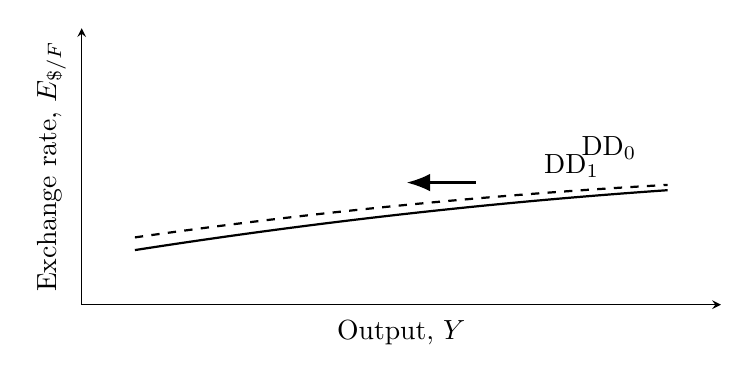
\begin{tikzpicture}
\begin{axis}[
  width=0.80\textwidth, height=0.42\textwidth,
  axis lines=left,
  xmin=0, xmax=12, ymin=0, ymax=12,
  xtick=\empty, ytick=\empty,
  xlabel={Output, $Y$},
  ylabel={Exchange rate, $E_{\$/F}$},
  clip=false
]

% Use gentle upward curves (almost linear) and a parallel left shift.
% DD0
\addplot[domain=1:11, samples=200, thick] {2.0 + 0.38*x - 0.010*x^2};
\node[anchor=west] at (axis cs:9.2,6.8) {$\dd_0$};

% DD1: left shift (equivalently, evaluate DD0 at x+1.6)
\addplot[domain=1:11, samples=200, thick, dashed] {2.0 + 0.38*(x+1.6) - 0.010*(x+1.6)^2};
\node[anchor=west] at (axis cs:8.5,6.0) {$\dd_1$};

% Shift arrow
\draw[-{Latex[length=3mm]}, thick]
  (axis cs:7.4,5.3) -- (axis cs:6.1,5.3);

\end{axis}
\end{tikzpicture}
\end{center}

\end{enumerate}
\end{problem}

% =========================================================
\begin{problem}{2}

\vspace{0.25em}
\begin{enumerate}[(a)]
\item \textbf{DD schedule for Japan.}

With short-run prices fixed, a rise in $E_{\yen/\usd}$ is a yen depreciation, which raises $\frac{EP^*}{P}$ and improves the current account,
increasing demand and output.

\begin{center}
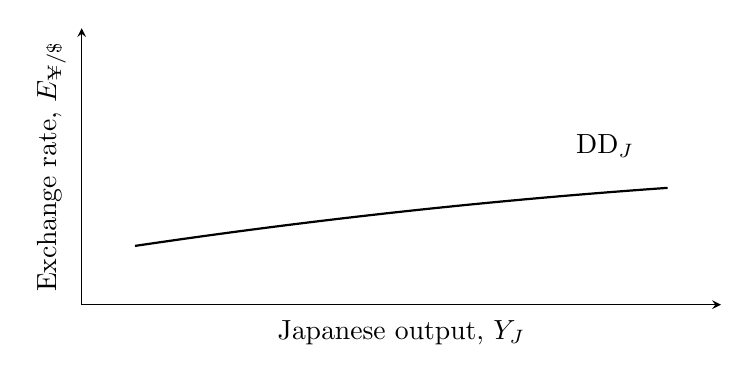
\begin{tikzpicture}
\begin{axis}[
  width=0.80\textwidth, height=0.42\textwidth,
  axis lines=left,
  xmin=0, xmax=12, ymin=0, ymax=12,
  xtick=\empty, ytick=\empty,
  xlabel={Japanese output, $Y_J$},
  ylabel={Exchange rate, $E_{\yen/\usd}$},
  clip=false
]
\addplot[domain=1:11, samples=200, thick] {2.2 + 0.36*x - 0.009*x^2};
\node[anchor=west] at (axis cs:9.1,6.9) {$\dd_J$};
\end{axis}
\end{tikzpicture}
\end{center}

\item \textbf{For each change, shift DD LEFT, RIGHT, or NO SHIFT.}

\[
D = C(Y-T) + I + G + \CA\!\left(\frac{EP^*}{P},\,Y-T\right).
\]
Any exogenous change that increases (decreases) demand for home goods shifts DD right (left).

\begin{enumerate}[(i)]
\item \textbf{Increase in Japanese government spending $G$:}
\[
G\uparrow \Rightarrow D\uparrow \Rightarrow \textbf{DD shifts RIGHT.}
\]

\item \textbf{Japanese consumers want to consume less/save more:}
\[
C()\downarrow \Rightarrow D\downarrow \Rightarrow \textbf{DD shifts LEFT.}
\]

\item \textbf{Exogenous increase in prices in Japan:}
\[
P\uparrow \Rightarrow \frac{EP^*}{P}\downarrow \Rightarrow \CA\downarrow \Rightarrow D\downarrow
\Rightarrow \textbf{DD shifts LEFT.}
\]

\item \textbf{Exogenous increase in the exchange rate $E_{\yen/\usd}$:}
Since $E_{\yen/\usd}$ is the axis variable, this is a \textbf{movement along DD (NO SHIFT).}

\item \textbf{Foreign sanctions reduce foreigners' propensity to buy Japanese goods:}
Exports fall at any real exchange rate, so $\CA$ shifts down:
\[
\CA\downarrow \Rightarrow D\downarrow \Rightarrow \textbf{DD shifts LEFT.}
\]
\end{enumerate}

\end{enumerate}
\end{problem}

\end{document}